\documentclass{article}

\usepackage{amsmath}
\usepackage{amssymb}
\usepackage{graphicx}

\usepackage[justification=centering]{caption}
\usepackage[font=footnotesize]{caption}

\newcommand{\noi}{\noindent}

\begin{document}

\begin{section}{State of the Implementation, 1/16/17}

The code, available in the ``code'' directory, contains much of the necessary framework for any algorithm which locates the optimal arrangement, as well as a number of attempted implementations of such an algorithm. (None of them work.) This document contains descriptions of the attempted implementations, as well as basic documentation of the existing code, which is also commented and should be fairly self-explanatory.

To begin using the code, see \S 3.1 for sample run commands.

\end{section}

\begin{section}{Attempted Implementations}

\begin{subsection}{MCMC Posterior Max}

The MCMC Posterior Max implementation is essentially an incomplete Markov chain Monte Carlo. We iteratively perturb the candidate strengths and positions (the ``outer loop'') and, for a given candidate arrangement, place each county optimally (the ``inner loop''). We accept these perturbations according to the Metropolis-Hastings criterion, and report the arrangements with the highest posterior probability.

In a true MCMC, we would interpret the set of all steps as a probability distribution of the true parameters and use some more intelligent process to identify our optimal choice of parameters. We would also have to run multiple threads in parallel to test for convergence. In the present implementation (which is not a true MCMC), we merely track the current best step.

Posterior probability in this implementation is calculated as follows:
\begin{align}
\text{posterior} &= \text{likelihood} \times \text{prior} \\
&= e^{-\text{EPE}} \times \prod_{K_i \in F} \ln \mathcal{N}(s_{K_i})
\end{align}

\noi That is, the likelihood decreases exponentially with total error, and our prior for an arrangement is a lognormal distribution on candidate strengths, to penalize cases where candidates have extremely high or low strengths. Strengths are normalized to a geometric mean of 1, so that e.g.\ the strengths $\{1,4,4,4\}$ and $\{\frac{1}{4},1,1,1\}$ are equivalent. There is presently no prior on positions, of candidates or counties.

The code for this implementation is in \texttt{optimize.py} under the heading \texttt{IMPLEMENTATION 1}. A sample run command for this implementation is:
\begin{verbatim}
    python main.py -d data/test_case_1.txt
                   -s solutions/test_case_1_solution.txt
                   -n 1000
                   --mcmc-posterior-max
\end{verbatim}


\end{subsection}

\begin{subsection}{``MCMC'' Error Min}

This is an old implementation and probably shouldn't be used, as MCMC Posterior Max is strictly better. The implementation is the same as above, with two differences:
\begin{enumerate}
\item There are no priors on candidate strengths.
\item We accept new steps deterministically (that is, not according to Metropolis-Hastings) based on whether the proposed new step has a lower EPE than the current step.
\end{enumerate}
Both of these elements are crucial to MCMC, and this implementation is something more like a simple gradient descent.

The code for this implementation is in \texttt{optimize.py} under the heading \texttt{IMPLEMENTATION 2}. A sample run command for this implementation is:
\begin{verbatim}
    python main.py -d data/test_case_1.txt
                   -s solutions/test_case_1_solution.txt
                   -n 1000
                   --mcmc-error-min
\end{verbatim}

\end{subsection}



\begin{subsection}{Scipy Minimize}

This implementation is very straightforward: we simply use the Scipy minimize function to find an optimal arrangement. Scipy uses a gradient descent, which falls into local minima very easily and thus does not give us the desired solution.

The only code involved in this implementation is used to convert candidate strengths and positions from formats we use to argument vectors which can be passed into Scipy minimize. The code for this implementation is in \texttt{optimize.py} under the heading \texttt{IMPLEMENTATION 3}. A sample run command for this implementation is:
\begin{verbatim}
    python main.py -d data/test_case_1.txt
                   -s solutions/test_case_1_solution.txt
                   -n 1000
                   --scipy-minimize
\end{verbatim}

\end{subsection}

\begin{subsection}{Scipy Basin-Hopping}

This implementation uses a slightly more sophisticated optimization technique, also provided by the Scipy package. The basin-hopping algorithm works like a simple gradient descent, with one modification: when a local minimum is identified, a large ``hop'' is taken and the gradient descent begins anew. This is used, generally speaking, to find global minima in situations where many local minima exist; however, I expect that there are too many local minima for a random hopping process like this to locate the global minimum.

In a number of test cases, this implementation is closest to finding the optimal arrangement. However, given that it is a pre-written package, we can't improve on its performance. The code for this implementation is in \texttt{optimize.py} under the heading \texttt{IMPLEMENTATION 4}. A sample run command for this implementation is:
\begin{verbatim}
    python main.py -d data/test_case_1.txt
                   -s solutions/test_case_1_solution.txt
                   -n 1000
                   --scipy-basinhopping
\end{verbatim}

\end{subsection}



\end{section}

\begin{section}{Code}

\begin{subsection}{Sample Run Commands}

Here is a simple run command, to run MCMC Posterior Max on a simple test case and write the best solution to a text file:
\begin{verbatim}
    python main.py -d data/test_case_1.txt
                   -s solutions/test_case_1_solution.txt
                   -n 100
                   --mcmc-posterior-max
\end{verbatim}

\noi If you run this command a second time, it should begin optimizing from the previous best solution (stored in the solution file passed in) and then write the new best solution over this same file.

Here is a run command to run MCMC Posterior Max on the same simple test case, writing the best solution to a text file and creating an image to visualize the solution it identified:
\begin{verbatim}
    python main.py -d data/test_case_1.txt
                   -s solutions/test_case_1_solution.txt
                   -n 100
                   --plot-all-counties images/test_case_1_viz.png
                   --mcmc-posterior-max
\end{verbatim}

Here is a run command to run MCMC Posterior Max on the same simple test case, writing the best solution to a text file and creating five images (every 20 iterations of the outer loop) to visualize the progression of solutions it is identifying:
\begin{verbatim}
    python main.py -d data/test_case_1.txt
                   -s solutions/test_case_1_solution.txt
                   -n 100
                   --plot-all-counties images/test_case_1_viz.png
                   --plot-every 20
                   --mcmc-posterior-max
\end{verbatim}

\end{subsection}

\begin{subsection}{Overview of Files}

Below is an overview of each of the files contained in the ``code'' directory:

\begin{itemize}
\item \texttt{config.py} contains logic for parsing command line arguments, and stores global variables used elsewhere e.g.\ \texttt{config.data\_file}.
\item \texttt{parse.py} contains the Election object as well as a function for converting data files into Election objects. Data files must be tab-separated 2D arrays with a single header row containing candidate names and a single header column containing county names. Optionally, data files can have counties separated into states, which take the form of rows with a state name in the header column and no data in the rest of the row. Here is a sample data file with no state separation:
\begin{verbatim}
                         Ann       Bob
               County 1  0.4       0.6
               County 2  0.5       0.5
               County 3  0.8       0.2
\end{verbatim}And here is one with:\begin{verbatim}
                         Ann       Bob
               State X
               County 1  0.4       0.6
               County 2  0.5       0.5
               State Y
               County 3  0.8       0.2
\end{verbatim}

\item \texttt{solution\_io.py} handles the reading and writing of solution files.
\item \texttt{optimize.py} contains all of the implementations of optimization techniques. This file contains the bulk of the code, and it is divided into a number of subsections with comment headers. At the top are the four implementations; next are general TURF helper functions; next are the two functions which run the ``inner loop'' used in all four implementations; next are helper functions for the two MCMC-based implementations; next and last are helper functions for the two Scipy-based implementations.
\item \texttt{main.py} mostly delegates to other files. It reads in the command line arguments, parses the data file and solution file (if provided), runs the appropriate optimization technique, saves the results, and generates a visualization (if requested).
\item \texttt{visualize.py} handles visualization logic. I have not gone through this file since it was originally written by Felix, so it isn't commented. I'll eventually go through and document this but for now, it works!
\end{itemize}
\end{subsection}

\begin{subsection}{Data}

I've been primarily using two data files: one test case, \texttt{test\_case\_1.txt}, and one real-world case, \texttt{super\_tuesday.tsv}.

The test case was generated by an Excel spreadsheet and has a theoretical solution with zero error (that is how it was generated, after all). The ``correct'' solution should look like this:
\begin{center}
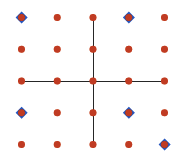
\includegraphics[width=0.4\textwidth]{test_case_1_theoretical_solution.png}
\end{center}
Here the red dots are the 25 counties, and the five blue diamonds are candidates named NorWest, NorEast, SouWest, SouEast (the four corners of the square), and Xxxx (the trailing candidate near SouEast). The optimal strengths for all candidates is 1. There seem to be other solutions with nearly zero error.

The real-world case contains data for every county that voted on Super Tuesday in the 2016 Republican Primary. The rows do not always add up to 1. There are many counties, so it may be useful to run with the \texttt{--num-counties} flag on to save on runtime.

\end{subsection}

\begin{subsection}{Miscellany}

There may be redundancies or errors in the code, which has not been thoroughly checked. For instance, we have not consistently used ``counties'' as I have in this document---there may be cases where ``voters'' is used instead.

A number of flags are not needed for running any implementation, but may be helpful for debugging. The flag \texttt{--fix-strength} holds all candidate strengths at 1, which is useful in implementations where strength varies wildly. Similarly, \texttt{--strength-scaling-factor} artificially reduces the variability of strength for similar cases. We hope that the addition of strength priors in MCMC Posterior Max obviates the need for these flags. The flag \texttt{--single-inner} runs one inner loop (for debugging purposes) and is not a fifth implementation, as it might seem.

\end{subsection}




\end{section}




\end{document}